\documentclass[a4paper]{article}

% \usepackage{inputenc}
\usepackage[british,UKenglish]{babel}
\usepackage{amsmath}
\usepackage{titlesec}
\usepackage{color}
\usepackage{graphicx}
\usepackage{fancyref}
\usepackage{hyperref}
\usepackage{float}
\usepackage{scrextend}
\usepackage{setspace}
\usepackage{xargs}
\usepackage{multicol}
\usepackage{nameref}

\usepackage{sectsty}
\usepackage{multicol}
\usepackage{multirow}
\usepackage[procnames]{listings}
\usepackage{appendix}
\usepackage{listings}

\newcommand\tab[1][1cm]{\hspace*{#1}}
\hypersetup{colorlinks=true, linkcolor=black}
\interfootnotelinepenalty=10000

\newcommand{\cleancode}[1]{\begin{addmargin}[3em]{3em}\texttt{\textcolor{cleanOrange}{#1}}\end{addmargin}}
\newcommand{\cleanstyle}[1]{\text{\textcolor{cleanOrange}{\texttt{#1}}}}


\usepackage[colorinlistoftodos,prependcaption,textsize=footnotesize]{todonotes}
\newcommandx{\commred}[2][1=]{\textcolor{Red}
{\todo[linecolor=red,backgroundcolor=red!25,bordercolor=red,#1]{#2}}}
\newcommandx{\commblue}[2][1=]{\textcolor{Blue}
{\todo[linecolor=blue,backgroundcolor=blue!25,bordercolor=blue,#1]{#2}}}
\newcommandx{\commgreen}[2][1=]{\textcolor{OliveGreen}{\todo[linecolor=OliveGreen,backgroundcolor=OliveGreen!25,bordercolor=OliveGreen,#1]{#2}}}
\newcommandx{\commpurp}[2][1=]{\textcolor{Plum}{\todo[linecolor=Plum,backgroundcolor=Plum!25,bordercolor=Plum,#1]{#2}}}

\def\code#1{{\tt #1}}

\def\note#1{\noindent{\bf [Note: #1]}}

\makeatletter
%% The "\@seccntformat" command is an auxiliary command
%% (see pp. 26f. of 'The LaTeX Companion,' 2nd. ed.)
\def\@seccntformat#1{\@ifundefined{#1@cntformat}%
   {\csname the#1\endcsname\quad}  % default
   {\csname #1@cntformat\endcsname}% enable individual control
}
\let\oldappendix\appendix %% save current definition of \appendix
\renewcommand\appendix{%
    \oldappendix
    \newcommand{\section@cntformat}{\appendixname~\thesection\quad}
}
\makeatother

\lstdefinelanguage{Julia}%
  {morekeywords={abstract,break,case,catch,const,continue,do,else,elseif,%
      end,export,false,for,function,immutable,import,importall,if,in,%
      macro,module,otherwise,quote,return,switch,true,try,type,typealias,%
      using,while,|>, .|>, =>, ->},%
   sensitive=true,%
   % alsoother={$},%
   morecomment=[l]\#,%
   morecomment=[n]{\#=}{=\#},%
   morestring=[s]{"}{"},%
   morestring=[m]{'}{'},%
}[keywords,comments,strings]%

\lstset{%
    language         = Julia,
    basicstyle       = \fontfamily{Fira Code},
    keywordstyle     = \bfseries\color{blue},
    stringstyle      = \color{magenta},
    commentstyle     = \color{ForestGreen},
    showstringspaces = false,
}




\lstset{frame=, basicstyle={\footnotesize\ttfamily}}



\graphicspath{ {images/} }
\usepackage{ctex}
\usepackage{fontspec}
% \usepackage[clean]{svg}
\setmonofont[
  Contextuals={Alternate}
]{Fira Code}
%-----------------------------------------BEGIN DOC----------------------------------------

\begin{document}
\renewcommand{\contentsname}{目\ 录}
\renewcommand{\appendixname}{附录}
\renewcommand{\appendixpagename}{附录}
\renewcommand{\refname}{参考文献} 
\renewcommand{\figurename}{图}
\renewcommand{\tablename}{表}
\renewcommand{\today}{\number\year 年 \number\month 月 \number\day 日}

\title{{\Huge 数据挖掘实验实验报告{\large\linebreak\\}}{\Large 实验一: 数据预处理\linebreak\linebreak}}
%please write your name, Student #, and Class # in Authors, student ID, and class # respectively
\author{\\姓\ 名:柴\ 博\ 文\\ 
学\ 号: 04194012\\
班\ 号: 大数据1901\\\\
数据挖掘与机器学习\\
(秋季, 2021)\\\\
西安邮电大学\\
计算机学院\\
数据科学与大数据专业}
\date{\today}
\maketitle
\newpage

%-----------------------------------------ABSTRACT-------------------------------------
\begin{center}
{\Large\bf{摘\ 要\\}}
\end{center}
本次实验使用Julia语言进行实现.

如果需要运行本项目代码,请安装python以及matplot

随后打开终端,运行Julia

安装XLSX,CSV,DataFrames,Plots,Dates,Statistics

实验报告采用LaTeX, 在overleaf上进行编写.

通过DataFrames, CSV, XLSX读取数据, PyPlots, Plots, StatsPlot绘制图案.

本次实验代码均可以在\href{https://github.com/lovebaihezi/lab/tree/main/data-process/lab1/julia}{github仓库}下找到.

\newpage
%-----------------------------------------CONTENT-------------------------------------
\begin{center}
\tableofcontents\label{c}
\end{center}
\newpage

%------------------------------------------TEXT--------------------------------------------

%----------------------------------------OVERVIEW-----------------------------------------

\section{概述} \label{overview}%------------------------------

1、掌握数据探索统计特征计算、数据可视化等基本方法

2、掌握数据集缺失值、含噪数据的平滑处理、数据变换、数据集成等预处理方法。

3、掌握PCA主成分分析等降维方法

\begin{itemize}
	\item{\textbf{数据可视化}对某县广电宽带用户的5000条数据(或者自己感兴趣的其他领域的数据)进行探索,通过统计特征可视化进行数据分析,探索发现你感兴趣的知识。}
    \item{\textbf{数据处理}对北京西安的年薪数据(或者自己感兴趣的其他领域的数据)计算均值,方差等统计特征,绘制据箱体图和小提琴图等图,分析北京西安年薪的差异。}
    \item{\textbf{数据清洗}用'movie\_metadata.csv'数据集(或者自己感兴趣的其他领域的数据)进行案例分析,这个数据集包含了包括演员、导演、预算、总输入,以及IMDB评分和上映时间等信息,进行处理缺失数据,可以是添加默认值,删除不完整的行,异常值处理,重复数据处理,规范化数据类型等等。
    }
    \item{\textbf{数据集成}合并两个给定数据集:ReaderRentRecode.csv和ReaderInformation.csv(或者自己感兴趣的其他领域的数据),其中两个数据集的共同点是具有相同的num属性,最终生成一个综合的数据集。
    }
    \item{\textbf{PCA}使用鸢尾花数据集(或者自己感兴趣的其他领域的数据),这个数据集有150个样本,其中每个样本有五个变量,其中四个为特征变量,分别为萼片长度(Sepal length), 萼片宽度(Sepalwidth),花瓣长度(Petallength),花瓣宽度(Petalwidth),还有一个变量是其所属的品种的类别变量(Species),这个鸢尾花内别共有3种类别分别是山鸢尾(Iris-setosa)、变色鸢尾(Iris-versicolor)和维吉尼亚鸢尾(Iris-virginica),首先对4维的原始数据集实现可视化,可视化一组数据来观察数据分布,然后对数据集进行标准化(归一化),接着利用PCA主成分分析将数据降到二维。}
\end{itemize}

%------------------------------------Lab Process--------------------------------------

\newpage
%------------------------------
\section{数据可视化}\label{sub:ptx}
\subsection{解析文件} \label{sub:ptxproc}

首先使用Excel讲旧版Excel格式的xls文件转换为CSV文件\href{"https://github.com/lovebaihezi/lab/blob/main/data-process/lab1/julia/file/xian_guangdian.csv"}{github}

随后使用CSV读取文件内容, 并通过DataFrame解析格式以及类型图\ref{fig:csvinfo}. 

\begin{figure}[ht]
 \centering
 \includegraphics[width=5cm]{images/广电信息CSV展示.png}
 \caption{广电信息CSV}
 \label{fig:csvinfo}
\end{figure}

\begin{lstlisting}[language=julia]
quality =
    "lab1/julia/file/xian_guangdian.csv" |>
    CSV.File |>
    DataFrame |>
    data ->
        begin
            combine(nrow, groupby(select(data, :客户等级), :客户等级)) |>
            data -> rename(data, :nrow => "用户数量") |> println
            combine(nrow, groupby(select(data, [:客户等级, :网络类型]), 
                                                [:客户等级, :网络类型]))
        end |>
        data ->
            rename(data, 
                :nrow => :quantity, 
                    :网络类型 => :net_kind, 
                        :客户等级 => :user_level)
data = combine(groupby(quality, :net_kind), [:user_level, :quantity])
dict = Dict(
    "5星ABD客户" => "star_5ABD",
    "离线" => "out_link",
    "3星AB客户" => "star_3AB",
    "1星D客户" => "star_1D",
    "1星A客户" => "star_1A",
    "VIP商业个人客户" => "vip",
    "3星AD客户" => "start_3AD",
)
1:(data|>nrow) .|>
i -> begin
    data[i, :net_kind] =
        Dict(
            "农网用户" => "village", 
            "城网用户" => "city",
            " " => "unknown"
        )[data[
            i,
            :net_kind,
        ]]
    data[i, :user_level] = dict[data[i, :user_level]]
end
gp = groupby(data, :net_kind)
gp |>
keys .|>
kind -> @df combine(gp[kind], [:user_level, :quantity]) plot(
    :user_level,
    :quantity,
    label = "$kind",
) |> fig -> savefig(fig, "lab1/julia/images/first_$kind")
\end{lstlisting}

\subsection{分组} \label{sub:group-1}

随后将数据根据客户等级进行分组,总共有7组,见图\ref{fig:customgroup}. 
\begin{figure}[ht]
 \centering
 \includegraphics[width=5cm]{images/广电客户.png}
 \caption{分组结果图}
 \label{fig:customgroup}
\end{figure}

再将每组一网络类型进行分组, 图\ref{fig:netgroup}. 

\begin{figure}[ht]
 \centering
 \includegraphics[width=5cm]{images/网络分组.png}
 \caption{分组结果图}
 \label{fig:netgroup}
\end{figure}

\subsection{绘制折线图} \label{sub:draw}

然后将每组画到折线图之上, 图\ref{fig:city}
\begin{figure}
    \centering
    \includegraphics[width=3cm]{images/city.png}
    \includegraphics[width=3cm]{images/village.png}
    \includegraphics[width=3cm]{images/unknown.png}
    \caption{城市居民, 农村, 未登记}
    \label{fig:city}
\end{figure}

\subsection{分析数据}\label{sub:ptxeva}

通过该次结果可以看出,在办理了广电业务的客户之中,5星ABD客户数目远远多余其他客户,而且明显城区用户多余农村用户

但是低级用户和高级用户的数量几乎差不多,而且最关键的是两个图的趋势是相似的,说明农村和城市对于网络的需求是很一致的

\newpage

% --------------------------------Evaluation----------------------------------------
\section{数据处理}\label{sub:process}
\subsection{求的统计数据} \label{sub:process-lab}

使用XLSX将文件内容读入,并使用DataFrame对数据进行类型判断并转换位DataFrame类型
随后使用统计模块中的统计方法求数据的均值,方差,标准差,协方差矩阵,图\ref{fig:mean}
在使用Plots进行绘图,图\ref{fig:violin_box}
\begin{lstlisting}[language=julia]
file_path = "lab1/julia/file/xian_beijing_salary.xlsx"
salarys = DataFrame(XLSX.readdata(file_path, 
                "Sheet1!C3:D14"), :auto) .|> identity
salary = [salarys.x1, salarys.x2]
println("mean:$(salary .|> Statistics.mean)")
println("var:$(salary .|> Statistics.var)")
println("std:$(salary .|> Statistics.std)")
println("cov:$(salary |> Statistics.cov)")
println("cor:$(salary .|> Statistics.cor)")
violin(["Xi'an"], salarys.x1, label = "Xi'an")
violin!(["Beijing"], salarys.x2, label = "Beijing")
boxplot(["Xi'an"], salarys.x1, label = "Xi'an")
boxplot!(["Beijing"], salarys.x2, label = "Beijing")
\end{lstlisting}

\begin{figure}[h]
    \centering
    \includegraphics[width=12cm]{images/数据处理.png}
    \caption{均值, 方差, 标准差, 协方差}
    \label{fig:mean}
\end{figure}
\subsection{绘制箱型图和小提琴图} \label{sub:violin-box}
\begin{figure}[h]
    \centering
    \includegraphics[width=6cm]{images/box.png}
    \includegraphics[width=6cm]{images/violin.png}
    \caption{箱型图和小提琴图}
    \label{fig:violin_box}
\end{figure}

\newpage

\section{数据预处理}\label{sub:pre_process}
\subsection{去除丢失数据行} \label{sub:pre_process-lab}

在读取完数据后,通过DataFrame转换之后

可以通过DataFrame得知
每一列都会有值是丢失的:图\ref{fig:movie_metadata}

\begin{figure}[h]
    \centering
    \includegraphics[width=12cm]{movie-metadata.png}
    \caption{电影元数据}
    \label{fig:movie_metadata}
\end{figure}

为了将来数据处理的正常话,这里将导演空的一栏都去掉
\subsection{默认值替换} \label{sub:default-data}
同时其他的值变为其默认值

\begin{table}[h]
    \centering
    \begin{tabular}{ |c|c| }
名称 & 默认值 \\\hline
color & Color \\ 
num critic for reviews & 0 \\ 
duration & 0 \\ 
director facebook likes & 0 \\ 
actor 3 facebook likes & 0 \\ 
actor 2 name & \ \\ 
actor 1 facebook likes & 0 \\ 
gross & 0 \\ 
genres & \ \\ 
actor 1 name & \ \\ 
movie title &   \\ 
num voted users & 0 \\ 
cast total facebook likes & 0 \\ 
actor 3 name &  \\
facenumber in poster & 0 \\ 
plot keywords &  \\ 
movie imdb link &  \\ 
    \end{tabular}
\end{table}

\newpage

\begin{table}[h]
    \centering
    \begin{tabular}{ |c|c| }
num user for reviews & 0 \\ 
language &  \\ 
country &  \\ 
content rating & PG-0 \\ 
budget & 0 \\ 
title year & 0 \\ 
actor 2 facebook likes & 0 \\ 
imdb score & 0 \\ 
aspect ratio & 0 \\ 
movie facebook likes & 0 \\ 
\end{tabular}
\end{table}

于是就对每一列进行一次变化:如果每一行的数据是missing,就将其替换为默认值,见图\ref{fig:missing}

\begin{figure}[h]
    \label{fig:missing}
    \centering
    \includegraphics[width=12cm]{去除导演missing的行.png}
    \includegraphics[width=12cm]{处理missing.png}
    \caption{处理missing}
\end{figure}

\begin{lstlisting}[language=julia]
\end{lstlisting}

\newpage

\section{数据合并}\label{sub:data_join}
\subsection{通过join进行合并} \label{sub:data_join-lab}

读取数据表,通过join表上的num列对两张表进行合并,图\ref{fig:combine}

\begin{figure}[h]
    \centering
    \includegraphics[width=12cm]{images/合并.png}
    \caption{数据合并}
    \label{fig:combine}
\end{figure}

\begin{lstlisting}[language=julia]
["lab1/julia/file/4ReaderInformation.csv",
     "lab1/julia/file/4ReaderRentRecode.csv"] .|>
CSV.File .|>
DataFrame |>
dates -> begin
    println(dates...)
    innerjoin(dates..., on = :num) |>
    file -> begin
        file |> println
        CSV.write("lab1/julia/file/join.csv", file)
    end
end
\end{lstlisting}

\newpage

\section{PCA}\label{sub:PCA}
\subsection{绘制四维图像} \label{sub:plot}
可视化四维数据,我对数据依据种类进行了分组,对每组进行了绘图

其中横轴,数轴,纵轴,颜色分别代表:萼片长度(Sepal length), 萼片宽度(Sepalwidth),花瓣长度(Petallength),花瓣宽度(Petalwidth)

\begin{figure}[ht]
    \centering
    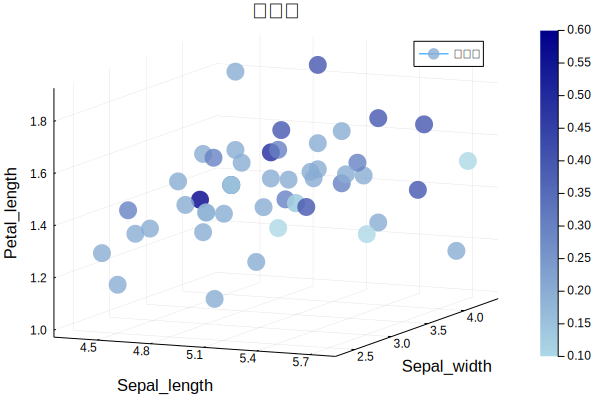
\includegraphics[height=5cm]{山鸢尾花.png}
    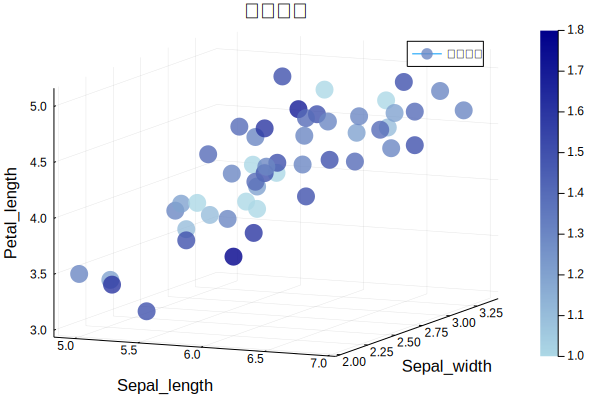
\includegraphics[height=5cm]{变色鸢尾花.png}
    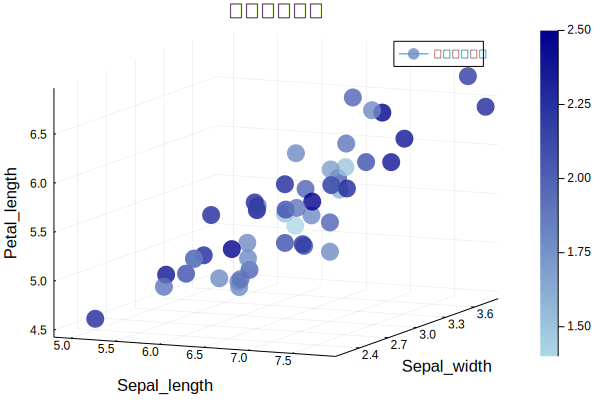
\includegraphics[height=5cm]{维吉尼亚鸢尾花.png}
    \caption{山鸢尾花,变色鸢尾花,维吉尼亚鸢尾花}
\end{figure}

\newpage

\subsection{实现PCA} \label{sub:PCA-}

PCA实现步骤

首先是算法思路
设有 $n$ 条 $d$ 维数据。
\begin{enumerate}
    \item 将原始数据按列组成 $n$ 行 $d$ 列矩阵 $X$
    \item 将 $X$ 的每一列(代表一个属性)进行零均值化,即减去这一列的均值
    \item 求出协方差矩阵 $\frac{1}{m}XX^T$
    \item 求出协方差矩阵的特征值及对应的特征向量
    \item 将特征向量按对应特征值大小从上到下按行排列成矩阵,取前 $k$ 行组成矩阵 $P$
    \item $Y=PX$ 即为降维到 $k$ 维后的数据
\end{enumerate}

\begin{lstlisting}[language=julia]

    data = copy(mat)
    data = select!(data, Not([:Species])) |> Matrix 
    (values, vectors) = data |> Statistics.cov |> eigen
    p = last(sortperm(values), 2) |> x -> vectors[:, x]
    data * p

\end{lstlisting}

\begin{figure}[ht]
    \centering
    \includegraphics{matrix.png}
    \caption{PCA结果}
    \label{fig:matrix}
\end{figure}

结果:图\ref{fig:matrix}

\newpage

% -----------------------------------Appendix----------------------------------------
\appendix
\section{代码}

\begin{lstlisting}[language=julia]
    using XLSX;
    using CSV;
    using DataFrames;
    using Plots;
    using Dates;
    using Statistics;
    using StatsPlots
    import PyPlot;
    using LinearAlgebra
    
    function free()
        quality =
            "lab1/julia/file/xian_guangdian.csv" |>
            CSV.File |>
            DataFrame |>
            data ->
                begin
                    combine(nrow, groupby(select(data, :客户等级), :客户等级)) |>
                    data -> rename(data, :nrow => "用户数量") |> println
                    combine(nrow, groupby(select(data, [:客户等级, :网络类型]), [:客户等级, :网络类型]))
                end |>
                data ->
                    rename(data, :nrow => :quantity, :网络类型 => :net_kind, :客户等级 => :user_level)
        data = combine(groupby(quality, :net_kind), [:user_level, :quantity])
        dict = Dict(
            "5星ABD客户" => "star_5ABD",
            "离线" => "out_link",
            "3星AB客户" => "star_3AB",
            "1星D客户" => "star_1D",
            "1星A客户" => "star_1A",
            "VIP商业个人客户" => "vip",
            "3星AD客户" => "start_3AD",
        )
        1:(data|>nrow) .|>
        i -> begin
            data[i, :net_kind] =
                Dict("农网用户" => "village", "城网用户" => "city", " " => "unknown")[data[
                    i,
                    :net_kind,
                ]]
            data[i, :user_level] = dict[data[i, :user_level]]
        end
        gp = groupby(data, :net_kind)
        gp |>
        keys .|>
        kind -> @df combine(gp[kind], [:user_level, :quantity]) plot(
            :user_level,
            :quantity,
            label = "$kind",
        ) |> fig -> savefig(fig, "lab1/julia/images/first_$kind")
    end
    
    function draw_plot()
        file_path = "lab1/julia/file/xian_beijing_salary.xlsx"
        salarys = DataFrame(XLSX.readdata(file_path, "Sheet1!C3:D14"), :auto) .|> identity
        salary = [salarys.x1, salarys.x2]
    
        println("mean:$(salary .|> Statistics.mean)")
        println("var:$(salary .|> Statistics.var)")
        println("std:$(salary .|> Statistics.std)")
        println("cov:$(salary |> Statistics.cov)")
        println("cor:$(salary .|> Statistics.cor)")
    
        violin(["Xi'an"], salarys.x1, label = "Xi'an")
        violin!(["Beijing"], salarys.x2, label = "Beijing") |>
        fig -> savefig(fig, "lab1/julia/images/violin")
        boxplot(["Xi'an"], salarys.x1, label = "Xi'an")
        boxplot!(["Beijing"], salarys.x2, label = "Beijing") |>
        fig -> savefig(fig, "lab1/julia/images/box")
    
    end
    
    function map_transform()
        file_path = "lab1/julia/file/3movie_metadata.csv"
        movie_metadata = file_path |> CSV.File |> DataFrame
        dropmissing!(movie_metadata, :director_name)
        dict = Dict(
            :color => "Color",
            :num_critic_for_reviews => 0,
            :duration => 0,
            :director_facebook_likes => 0,
            :actor_3_facebook_likes => 0,
            :actor_2_name => "",
            :actor_1_facebook_likes => 0,
            :gross => 0,
            :genres => "",
            :actor_1_name => "",
            :movie_title => "",
            :num_voted_users => 0,
            :cast_total_facebook_likes => 0,
            :actor_3_name => "",
            :facenumber_in_poster => 0,
            :plot_keywords => "",
            :movie_imdb_link => "",
            :num_user_for_reviews => 0,
            :language => "",
            :country => "",
            :content_rating => 0,
            :budget => 0,
            :title_year => 0,
            :actor_2_facebook_likes => 0,
            :imdb_score => 0,
            :aspect_ratio => 0,
            :movie_facebook_likes => 0,
        )
        dict |>
        keys .|>
        key -> transform!(
            movie_metadata,
            :,
            key => (col -> col .|> each -> if ismissing(each)
                Dict[key]
            else
                each
            end) => key,
        )
    end
    
    function join_compine()
        ["lab1/julia/file/4ReaderInformation.csv", "lab1/julia/file/4ReaderRentRecode.csv"] .|>
        CSV.File .|>
        DataFrame |>
        dates -> begin
            println(dates...)
            innerjoin(dates..., on = :num) |>
            file -> begin
                file |> println
                CSV.write("lab1/julia/file/join.csv", file)
            end
        end
    end
    
    function self_pca()
        mat = "lab1/julia/file/5iris.csv" |> CSV.File |> DataFrame
        gp = groupby(mat, :Species)
        names = [:Sepal_length, :Sepal_width, :Petal_length, :Petal_width, :Species]
        @df gp[1] plot(
            :Sepal_length,
            :Sepal_width,
            :Petal_length,
            zcolor = reverse(:Petal_width),
            m = (10, 0.8, :blues, Plots.stroke(0)),
            fontfamily = "Yahei",
            xlabel = "Sepal_length",
            ylabel = "Sepal_width",
            zlabel = "Petal_length",
            title = "山鸢尾",
            label = "山鸢尾",
            w = 0,
        )
        @df gp[2] plot(
            :Sepal_length,
            :Sepal_width,
            :Petal_length,
            zcolor = reverse(:Petal_width),
            m = (10, 0.8, :blues, Plots.stroke(0)),
            fontfamily = "Yahei",
            xlabel = "Sepal_length",
            ylabel = "Sepal_width",
            zlabel = "Petal_length",
            title = "变色鸢尾",
            label = "变色鸢尾",
            w = 0,
        )
        @df gp[3] plot(
            :Sepal_length,
            :Sepal_width,
            :Petal_length,
            zcolor = reverse(:Petal_width),
            m = (10, 0.8, :blues, Plots.stroke(0)),
            fontfamily = "Yahei",
            xlabel = "Sepal_length",
            ylabel = "Sepal_width",
            zlabel = "Petal_length",
            title = "维吉尼亚鸢尾",
            label = "维吉尼亚鸢尾",
            w = 0,
        )
        data = copy(mat)
        data = select!(data, Not([:Species])) |> Matrix 
        (values, vectors) = data |> Statistics.cov |> eigen
        p = last(sortperm(values), 2) |> x -> vectors[:, x]
        data * p
    end
    
    free();
    draw_plot();
    map_transform();
    join_compine();
    self_pca();
    
\end{lstlisting}
\end{document}

